%
% !TeX root =./main.tex
% !TeX spellcheck = en_US

We base our study on data that is available from OSM \cite{OpenStreetMap}.
We use the \emph{R} programming language \cite{RVienna} to extract that data from
\emph{Overpass} API we use the \texttt{osmdata} R package \cite{osmdataR20221}.


\subsection{Road Network and Levels}
To get the road network we query the OSM \texttt{key}$=$\textit{highway}. We consider the
assigned values indicate the importance of the highway within the road network.
This classification is typically highly correlated to the official (legal) classification
but is not obligated to adhere to them. In our analysis we consider the
\texttt{values}$=$
\textit{'motorway', 'trunk', 'primary', 'secondary', 'tertiary', 'motorway\_link', 'trunk\_link', 'primary\_link', 'secondary\_link', 'tertiary\_link'}

\subsection{Maximum Road Gradients}

\begin{figure}[!ht]
  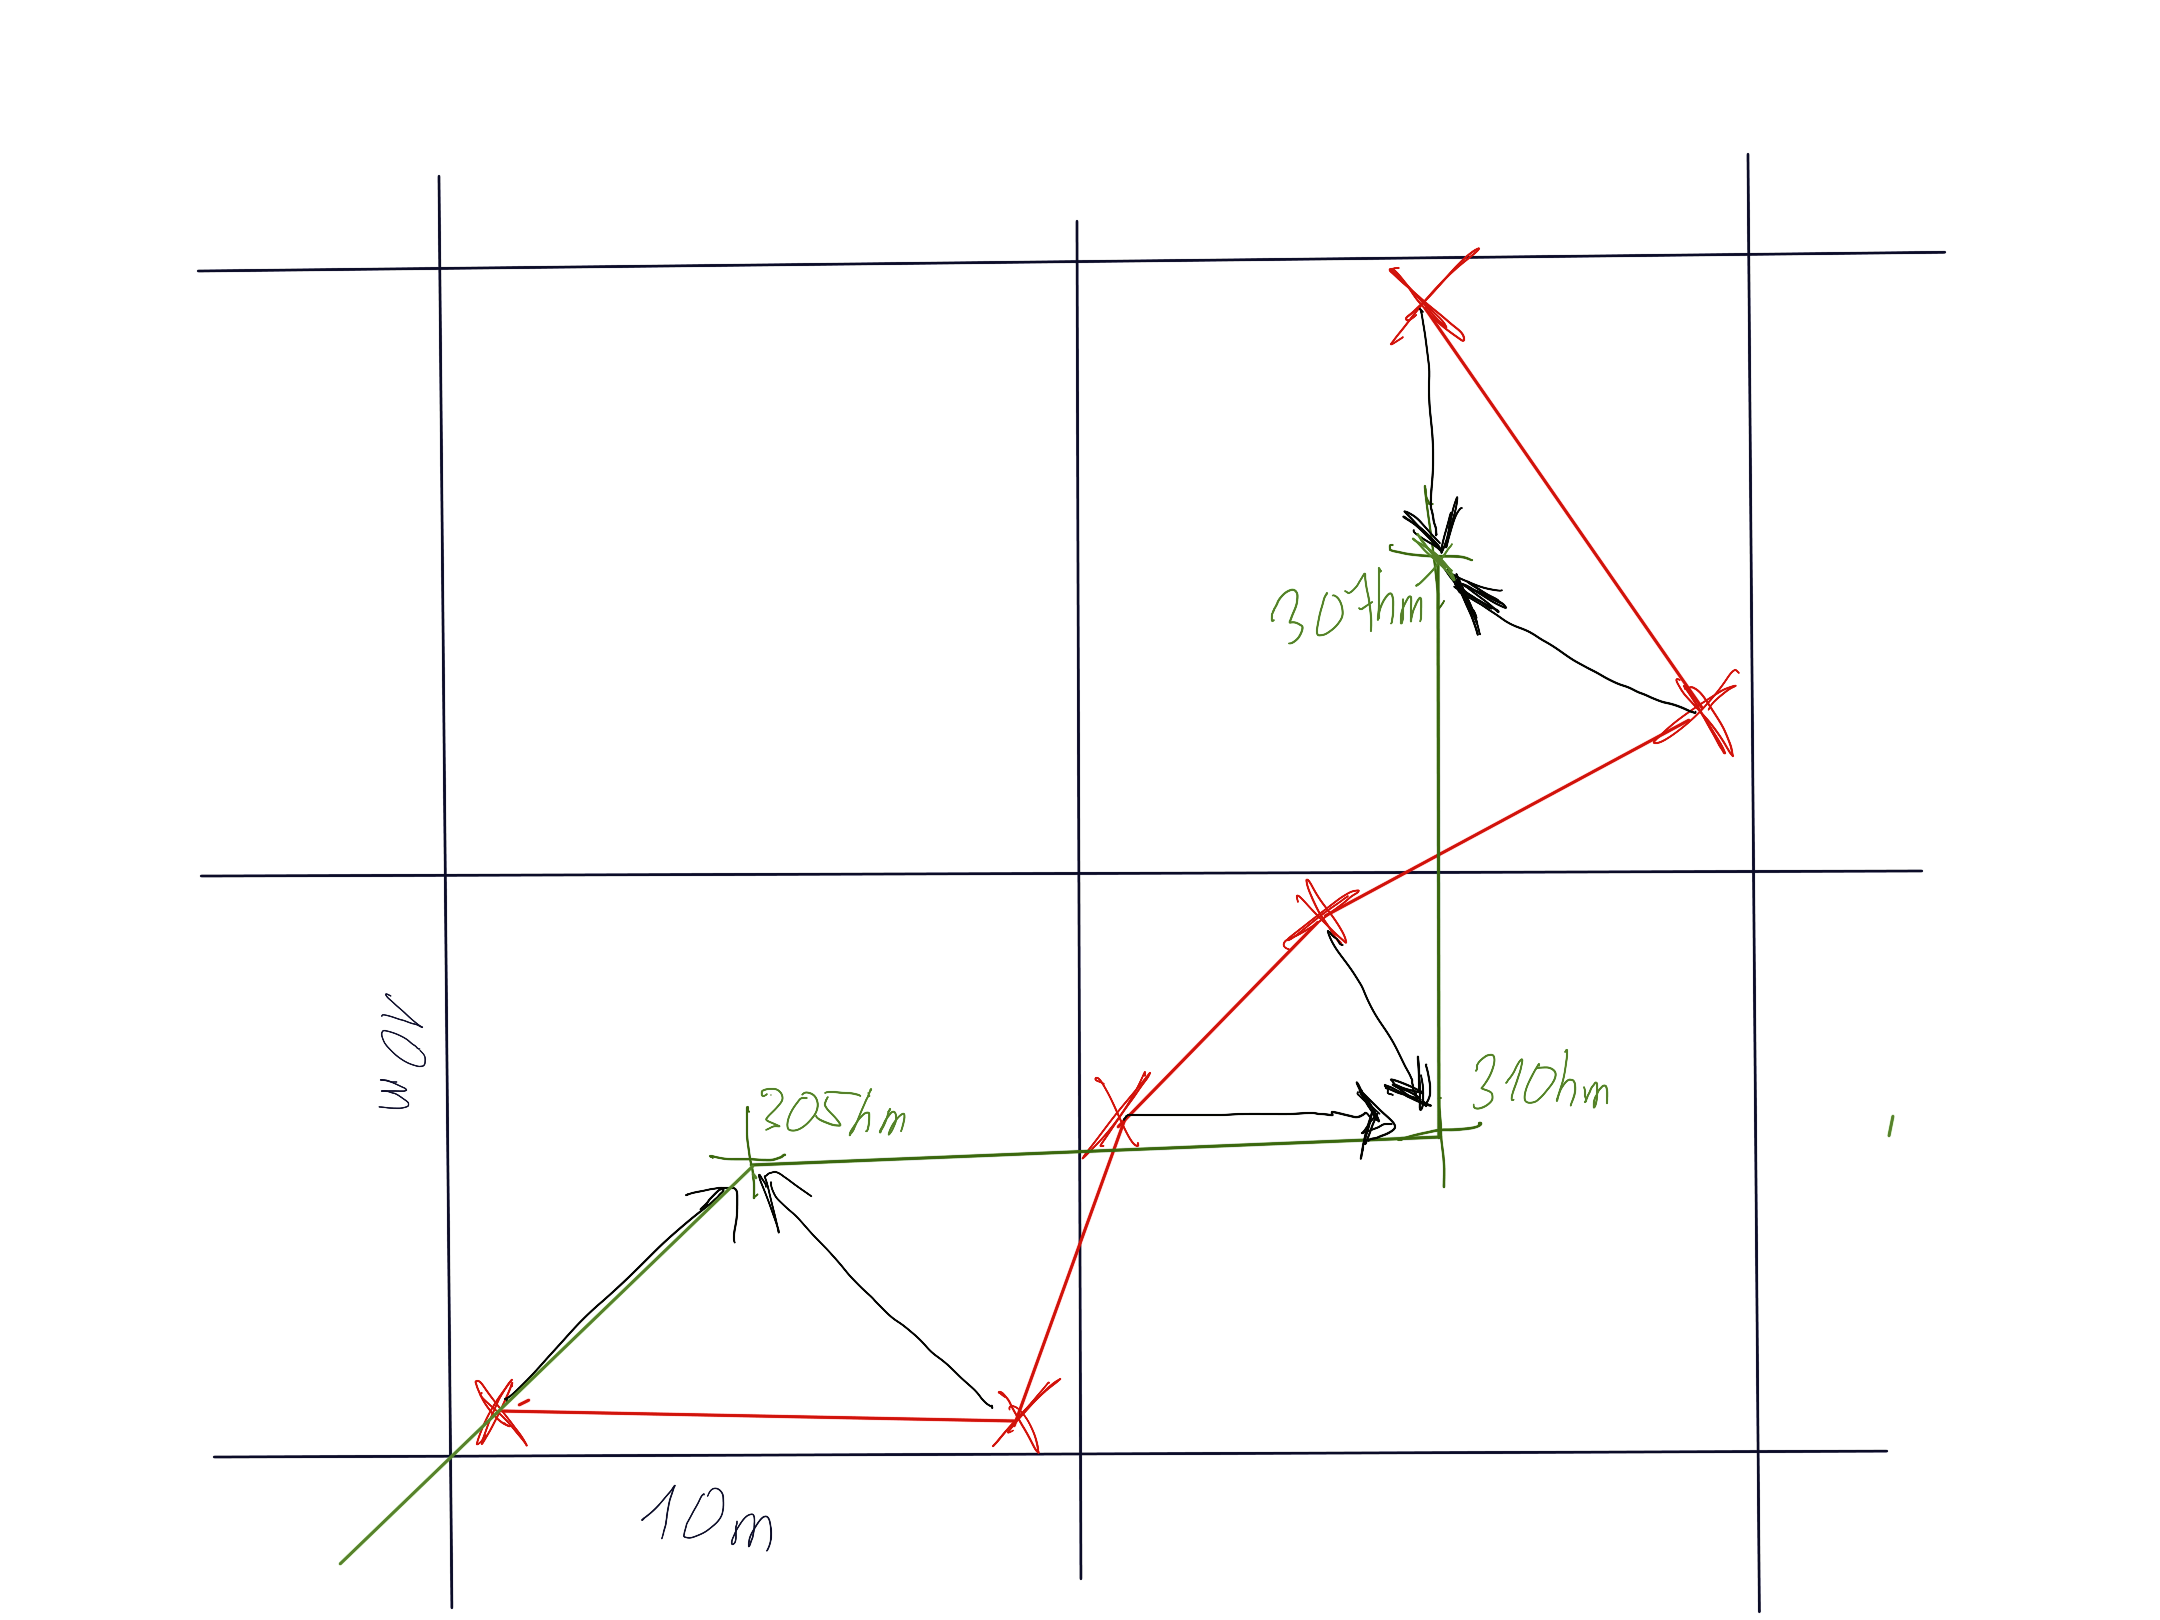
\includegraphics[width=0.9\textwidth]{./figures/mapping.png}
  \caption{Illustration of how a linestring is mapped to the grid that gives the elevation data.}
  \label{fig:mapelev}
\end{figure}
% https://civilnoteppt.com/6-types-of-classification-of-gradient-ruling-limiting-exceptional-minimum-average-and-floating-gradient/
% https://www.civillead.com/road-gradient/


\subsection{Bridge Weight Capacities}
Bridges are extracted by querying the \texttt{key}$=$\textit{bridge}. The tag \textit{maxweight}
tells as the maximal carrying capacity of the bridge. In case that no the field is empty,
following the rule of thump, there is now restriction for road legal vehicles, and
a weight restriction of $60t$ (or more is assumed).
We map the bridges to the road segment using the \texttt{???} package.
